\documentclass[11pt]{article}
\usepackage[a4paper,margin=1in]{geometry}
\usepackage[utf8]{inputenc}
\usepackage[T1]{fontenc}
\usepackage{microtype}
\usepackage{amsmath,amssymb}
\usepackage{booktabs}
\usepackage{graphicx}
\usepackage[hidelinks]{hyperref}

\title{\textbf{Placing a Migration's Tables into a Diagram Somebody Already Arranged}}
\author{Vasili Gavrilov\thanks{Independent researcher. Library, data and every number's
script: \url{https://github.com/Anode1/cjitter}, directory \texttt{example/erd}.}}
\date{Draft, August 2026}

\begin{document}
\maketitle

\begin{abstract}
A quality metric that cannot tell a person's careful work from a random draw is not
measuring the drawing. Straight-line stress is such a metric for entity-relationship
diagrams, and it is what every library offering frozen placement optimises. On a real
44-table diagram it scores the maintainer's own arrangement at 218{,}207 and uniform random
placement at 219{,}319, within one per cent: indistinguishable. Score the orthogonal
connector the diagram actually draws and the same two layouts separate by a factor of two,
157{,}552 against 80{,}606. We give that objective, a C library that optimises it with a
matched-budget random control in the API, and a benchmark of sixteen consecutive migrations
of one production schema over seven months. Freezing a subset is not new, and we claim
none of it: it is the stability term of Brandes and Wagner, the pinning weight of Frishman
and Tal, and it ships in Graphviz, ELK, NetworkX, d3-force, draw.io and yFiles. What is new
is the edge model, and the finding that it, rather than the search, decides the answer.
\end{abstract}

\section{A metric that cannot see the drawing}

Figure~\ref{fig:models} is one diagram under two edge models. The same 44 boxes sit in the
same places in both. On the left the edges are straight centre-to-centre segments; on the
right they are the orthogonal connectors the editor draws and the reader sees.

\begin{figure}[h]\centering
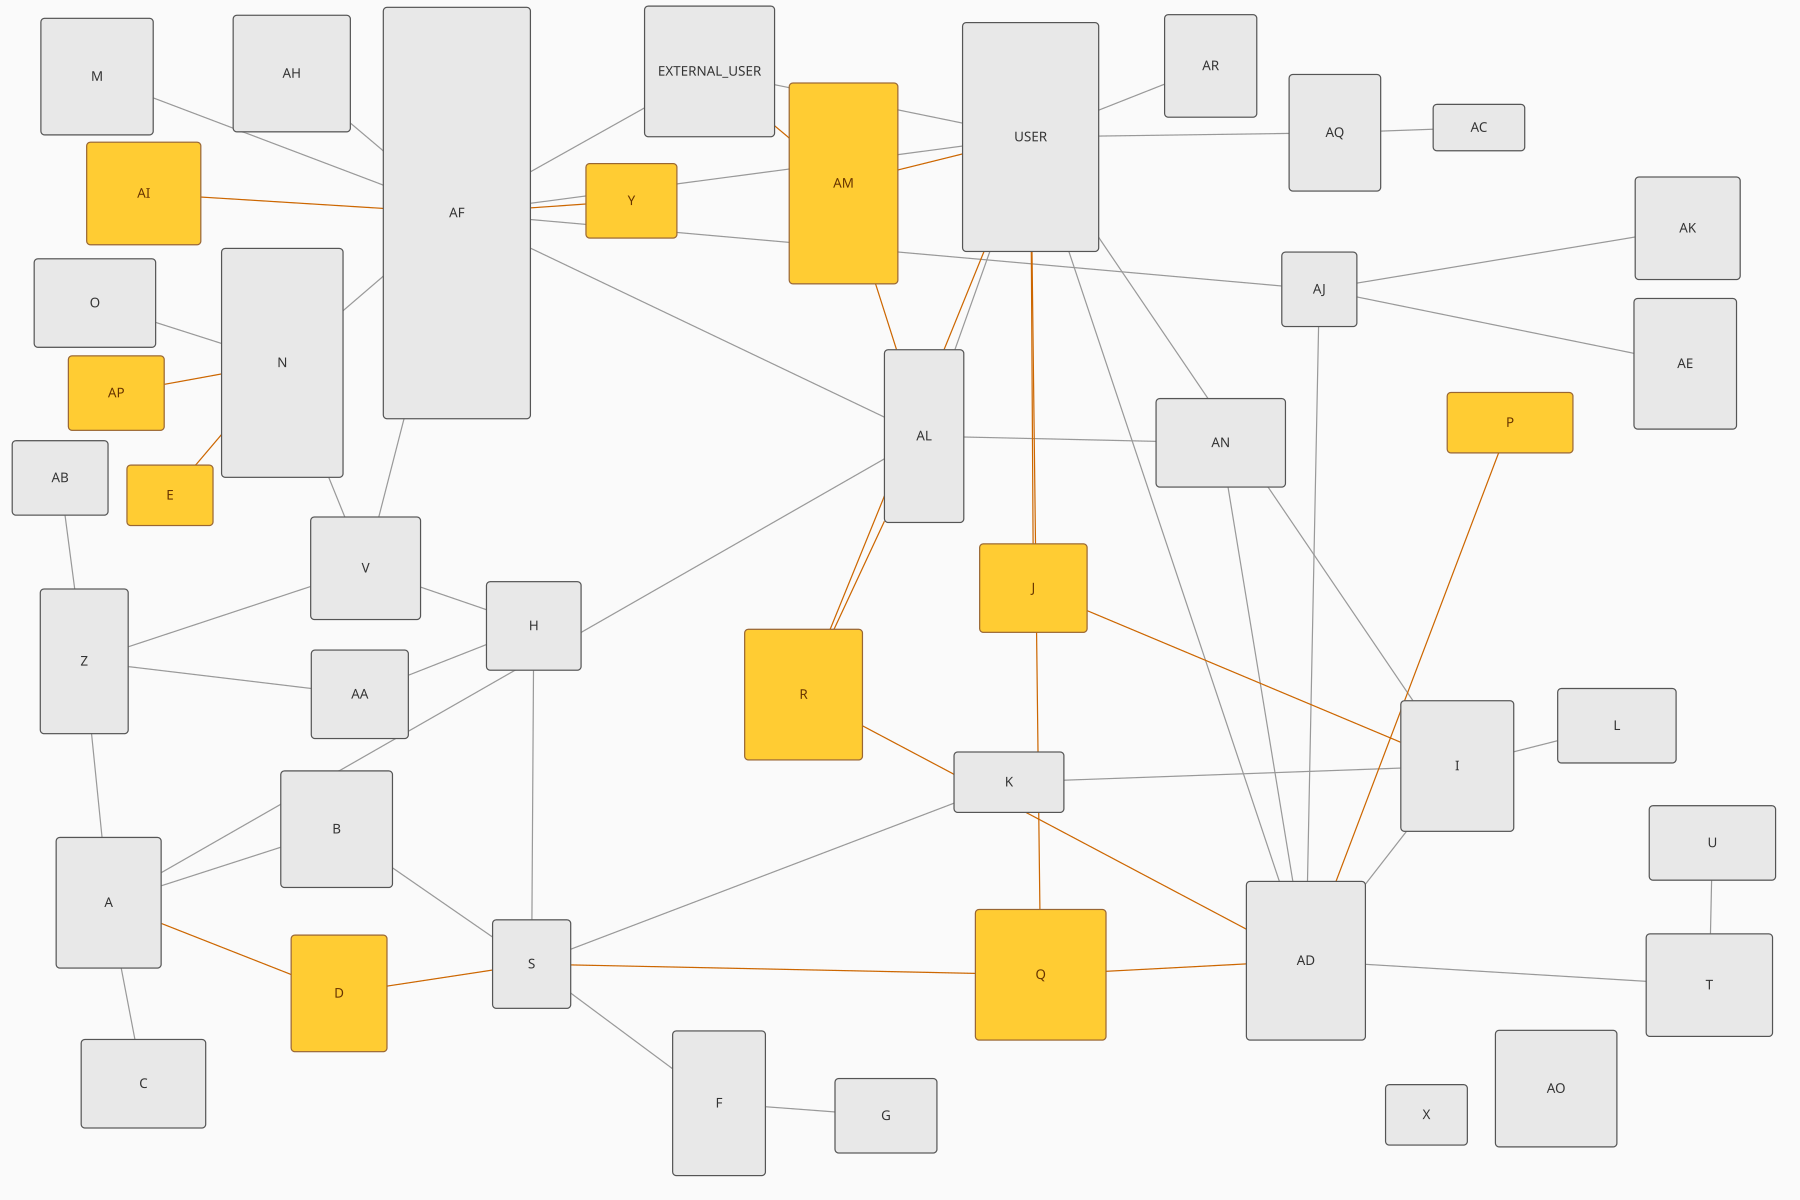
\includegraphics[width=0.47\textwidth]{figures/ERD_straight.png}\hfill
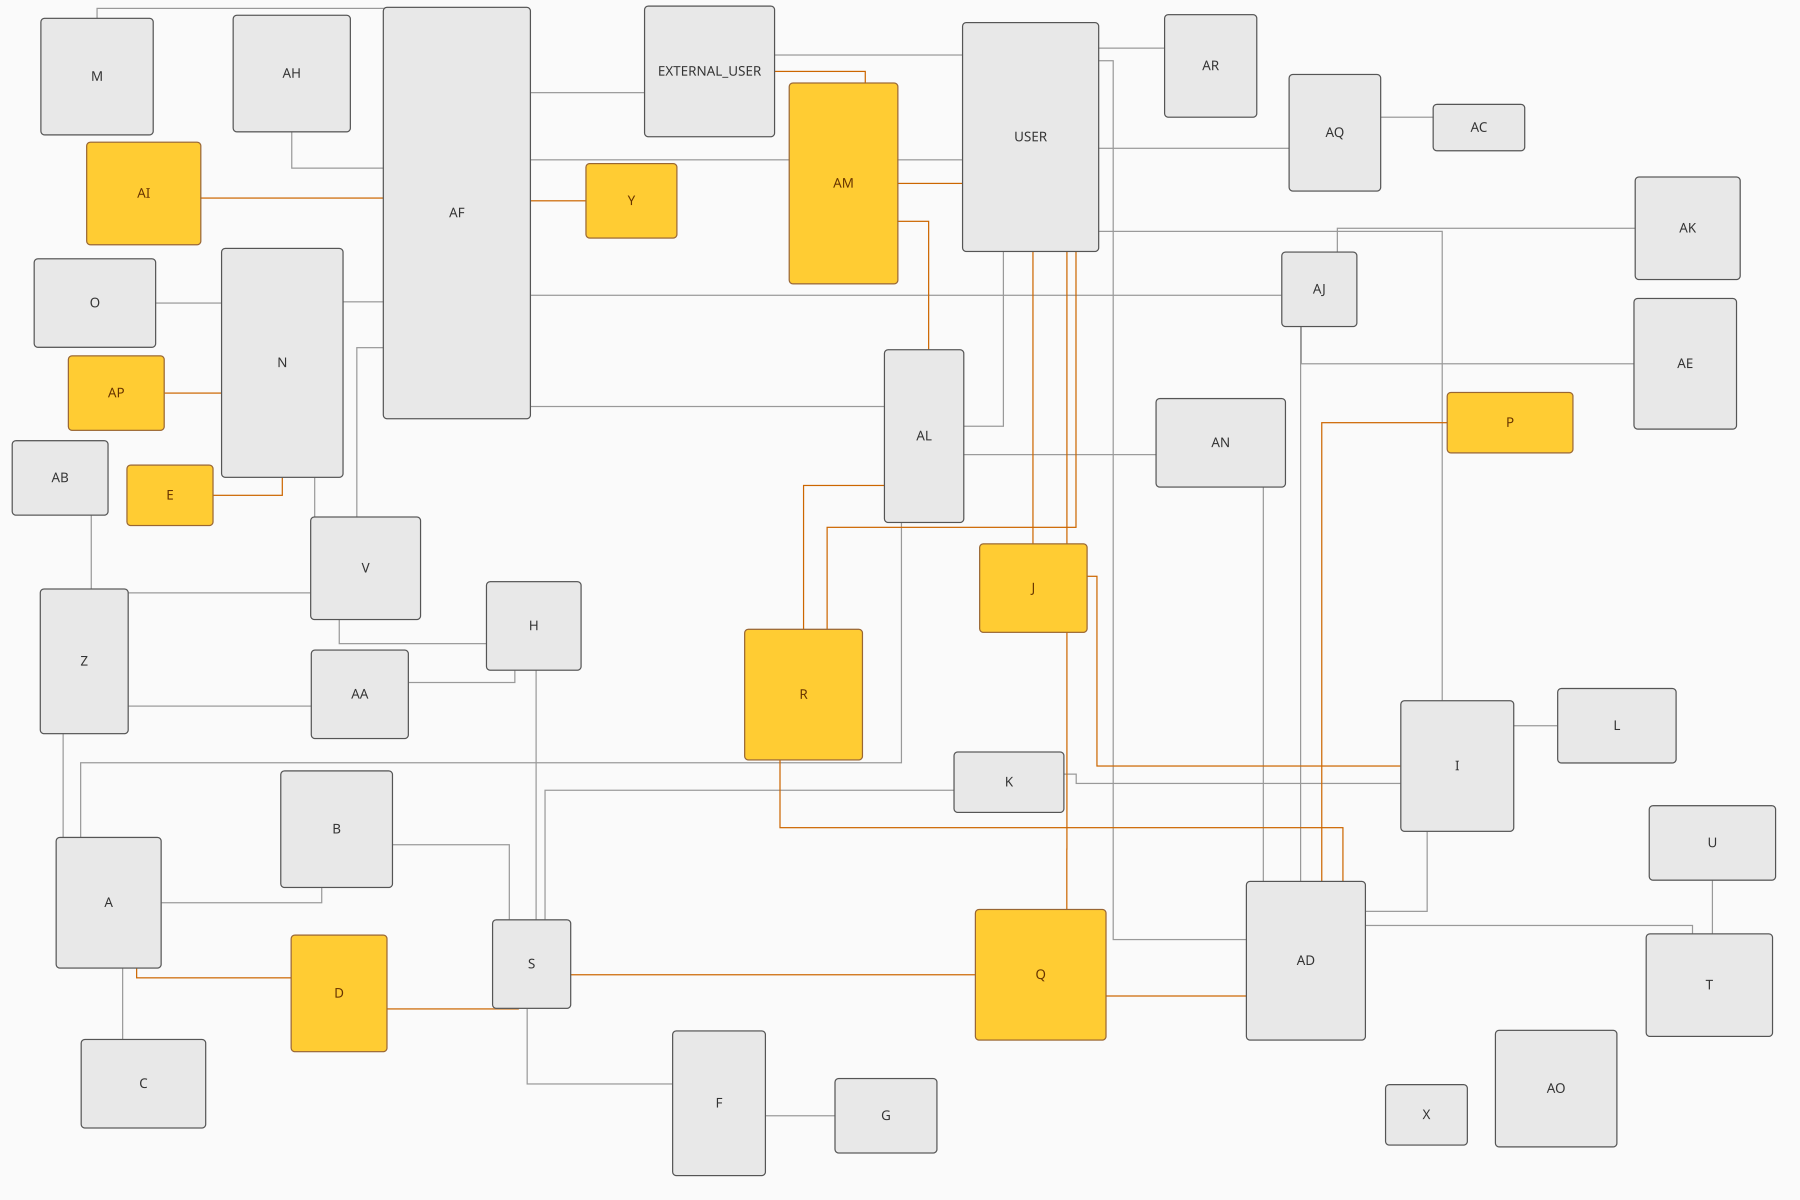
\includegraphics[width=0.47\textwidth]{figures/ERD_routed.png}
\caption{One production schema, 44 tables, 59 foreign keys, identical coordinates. Left,
straight centre-to-centre edges, the representation every frozen-placement library scores.
Right, the orthogonal routed connectors the editor draws. The ten tables the last migration
added are in amber. Under the left model this arrangement scores 218{,}207 and a uniform
random placement of the same ten tables scores 219{,}319; under the right model, 157{,}552
against 80{,}606.}
\label{fig:models}
\end{figure}

Calibrate each model against the one certain fact about this arrangement: on screen it has
no crossing and no edge running under a table. The straight model charges that clean screen
20 crossings and 1944 units of penetration. The routed model charges it 27 and 323. The
straight model is inventing more than a thousand units of a defect the reader cannot see,
because it draws diagonals through boxes that the editor routes around.

That is why it ranks a maintained diagram level with a random one. The consequence for
anyone building layout on top of such a metric is direct: the search can be excellent and
the answer still wrong, because the thing being minimised is not the thing being read.

\section{Where the problem arises}
A production schema under version control, 44 tables on its diagram and 59 foreign keys
drawn between them, gained ten tables in one migration. The maintainer had arranged the
other 34 by hand over seven months. Two things can happen to that arrangement, and both
cost the maintainer an hour.

The tools offer one command each. MySQL Workbench's is documented in full as
``Autolayout: Automatically arranges objects on the canvas'': no scope, no parameters, no
way to hold a table where it is. Oracle SQL Developer Data Modeler's is ``AutoLayout:
Rearranges the objects in the diagram'', and its manual's remedy for a bad result is Undo.
Neither product documents what becomes of hand-placed positions when the model is
refreshed from the database, and Workbench's reverse-engineering builds a \emph{new}
auto-placed diagram rather than merging into the existing one. Across nineteen database
diagram tools we checked, no vendor states what happens to a hand-made arrangement on
refresh. Three (SAP PowerDesigner, erwin, Visio) already scope layout to a selection.

The cost is measurable, and the schema's own history measures it. Seventeen revisions of
one \texttt{.mwb} file in git, sixteen consecutive migrations between November 2025 and
June 2026, the diagram growing from 15 to 44 tables:

\begin{center}\small
\begin{tabular}{lrrrrrrrr}
\toprule
revision & r02 & r05 & r06 & r07 & r12 & r14 & r16 & r17 \\
\midrule
moved, of tables kept & 15/15 & 14/14 & 0/15 & 15/15 & 15/15 & 18/18 & 19/19 & 19/19 \\
median shift & 82 & 924 & 0 & 168 & 42 & 26 & 1000 & 1544 \\
\bottomrule
\end{tabular}
\end{center}

In twelve of the sixteen migrations every retained table changed position. We report this
as the size of the problem and not as a measurement of either tool: the file records that
positions moved, not who moved them, and the zero rows show the churn is not automatic.
Separating the tool from the maintainer's own editing needs the refresh reproduced, which
we have not done.

\section{What was done before us}

The method is not ours and we do not claim it. Brandes and Wagner \cite{bw97} put dynamic
layout as a product of a readability term and a stability term; Brandes and Mader
\cite{bm11} write the stress form of it as
\begin{equation}
\mathrm{stress}_\alpha(P) = (1-\alpha)\,\mathrm{stress}(P)
  \;+\; \alpha \sum_{i \in V} \varphi_i \, \lVert p_i - \bar p_i \rVert^2 ,
\label{eq:anchor}
\end{equation}
with per-vertex tolerance weights $\varphi_i$. Holding a subset exactly is the
$\varphi_i \to \infty$ limit of~\eqref{eq:anchor} on that subset. Frishman and Tal
\cite{ft08} named the operation: a node's \emph{pinning weight} of 1 fixes it during layout
and 0 leaves it free. Coleman and Parker \cite{cp96} had already stated the goal, that
existing nodes should change as little as possible when the graph changes.

It ships, hard and per node, in most of the field:

\begin{center}\small
\begin{tabular}{@{}lll@{}}
\toprule
system & mechanism & edges \\
\midrule
Graphviz \texttt{neato}, \texttt{fdp} & \texttt{pin=true} with \texttt{pos} & straight \\
ELK stress & \texttt{org.eclipse.elk.stress.fixed} & straight \\
NetworkX & \texttt{spring\_layout(pos=\ldots, fixed=\ldots)} & straight \\
d3-force & \texttt{node.fx}, \texttt{node.fy} & straight \\
cytoscape.js-fcose & \texttt{fixedNodeConstraint} & straight \\
MSAGL & \texttt{CreateLock}, a continuous stay weight & straight \\
draw.io & \texttt{respectFixedPosition}, default true & orthogonal, unscored \\
Visio & \texttt{ShapeFixedCode = \&H1} & orthogonal, unscored \\
yFiles & \texttt{PartialLayouter} & orthogonal, unscored \\
\bottomrule
\end{tabular}
\end{center}

yFiles states our use case in its own documentation: changing the coordinates of partial
elements only, for applications where users incrementally add elements to an existing
drawing. Anyone who needs frozen placement and can take a Java or JavaScript dependency is
already served.

Whether preserving an arrangement helps a reader is not settled in general. Most experiments
found nothing: Archambault and Purchase report no significant difference in response time or
error rate \cite{ap12}, and their survey concludes no experiment had then found conclusive
evidence \cite{ap13}. The exception is the case here. On tasks of orienting oneself and
finding specific locations, with five or more targets and no colour cue, they find
preservation significantly faster and less error-prone \cite{ap12gd}. A 44-table diagram
somebody navigates from memory is that case, not the animated-sequence case the null results
studied.

\section{The math}

\paragraph{The problem.} A diagram is $n$ boxes of fixed size. The first $f$ are frozen at
the coordinates a person chose; the remaining $k = n - f$ are placed. With
$E_w = \sum_j w_j T_j$ a weighted sum of the usual criteria, the search is
\begin{equation}
\min_{\,x \in \mathbb{R}^{2k}} E_w\big(x \,\big|\, \bar x_{1:f}\big),
\end{equation}
the energy restricted to the free coordinates with the frozen ones substituted as
constants. Three consequences, and the third is a limitation.

\paragraph{Stability is exact.} Frozen boxes are not variables, so their displacement is
zero for every candidate the search ever scores. This is trivial as mathematics and it is
the whole guarantee a maintainer wants: it is the property the two products do not offer.

\paragraph{Dimension falls, and it buys budget.} On the diagram here, $2n = 88$ free
variables become $2k = 20$. If a good region occupies a fraction $\rho$ of each box's range,
its volume is $\rho^{n}$ against $\rho^{k}$, so the evaluations a sampling method needs for
a fixed success probability fall exponentially in the number of boxes frozen. Measured, on
30 rectangles at 28\% area coverage, 8{,}000 evaluations, 101 seeds, median residual
overlap: uniform sampling leaves 14.57 with 10 free and 121.34 with 30 free. A hill climber
leaves 0.00 in both. So the dimension argument is real for sampling and does not by itself
justify freezing for quality; at these densities a local search does not need the help.
Freezing is justified by the stability above, not by this.

\paragraph{A minimum of the restriction is not a minimum of the whole.} Substituting
constants can only raise the attainable minimum, and the point found is stationary in the
free coordinates alone. Freezing trades global optimality for the maintainer's map. That is
the trade the maintainer is asking for, and it should be stated rather than assumed away.
Exactness is not on the table in any case: minimising crossings alone is NP-complete
\cite{gj83}, so every tool here runs heuristics and the comparison is between them.

\section{The measurement}

The objective scores the routed geometry directly: each edge is an L or a Z whose middle
segment slides across the channel, routed against the frozen diagram once and against the
placed tables at every evaluation. Scores of the 44-table diagram of
Figure~\ref{fig:models}, 15 seeds, 8{,}000 evaluations, beside the library's own
matched-budget control:

\begin{center}\small
\begin{tabular}{lrrr@{\hspace{18pt}}rrr}
\toprule
& \multicolumn{3}{c}{straight diagonal edges} & \multicolumn{3}{c}{orthogonal routed connectors} \\
\cmidrule(r){2-4}\cmidrule{5-7}
 & median & wins & Holm $p$ & median & wins & Holm $p$ \\
\midrule
centroid rule    & 215{,}066 & & & 187{,}368 & & \\
the maintainer   & 218{,}207 & & & 157{,}552 & & \\
random (control) & 219{,}319 & & & 80{,}606 & & \\
climb            & 90{,}661 & 15/15 & 9.2e-5 & 46{,}852 & 15/15 & 9.2e-5 \\
anneal           & 104{,}482 & 15/15 & 9.2e-5 & 46{,}637 & 15/15 & 9.2e-5 \\
ga               & 72{,}766 & 15/15 & 9.2e-5 & 39{,}561 & 15/15 & 9.2e-5 \\
\bottomrule
\end{tabular}
\end{center}

Under straight edges the maintainer, the centroid rule and uniform random placement are
within 2\% of each other: the model cannot tell a hand-made arrangement from a random one.
Under routed edges they separate by a factor of two. A frozen-placement library that scores
straight lines is measuring something the reader never sees.

The second finding is against us and we report it as such. Under the routed model every
search beats the maintainer, 46{,}852 against 157{,}552 for the climber. We do not read that
as better layouts. We read it as the objective missing what the maintainer optimised, and we
treat the human score as a reference line rather than a target. An objective that ranks a
person's careful work below a hill climber's is incomplete, whatever it scores.

\section{What we offer}

A C library of four searches over a box of reals, with no dependency beyond \texttt{libm},
deterministic byte for byte from a seed on any compiler and platform. Two properties are
unusual and both matter here.

The control is in the API. \texttt{cjitter\_compare} runs uniform sampling at the same
budget on the same seeds as the method under test and prints the per-seed wins, the exact
one-sided sign test and its Holm-corrected probability across the methods compared. A
verdict of ``better'' is declared only at or under 5\% after correction, and a failure to
separate is printed as ``not shown'' and never as equality. The table above is that output.

Every method constant is a caller-visible field read literally, so an ablation is a value
and not a rebuild. One of them matters for this problem. \texttt{block} is how many
variables a proposal moves; at the default the whole migration moves at once, so a proposal
that seats one table beside its neighbour usually unseats another and is rejected for it. At
\texttt{block} 2 the same climb accepts 158 proposals instead of 42 and finishes 31\% lower,
32{,}428 against 46{,}665.

\section{What we suggest}

To the two vendors: give the existing command a scope. The mechanism is a boolean per
figure and it exists in draw.io, Visio, Gephi and yFiles already. Workbench needs no new
file format for it: the GRT tree exposes
\texttt{wb.doc.physicalModels[0].diagrams[0].figures} to Python plugins, so a layout can
read and write figure geometry from a plugin directory. What it lacks is a documented
figure geometry attribute set and any statement of what refresh does to positions.

To anyone building frozen placement: score the edge you draw. If the diagram draws
orthogonal connectors, straight-line stress will rank a hand-made arrangement level with a
random one, as it does above.

To ourselves: the churn in section 1 is not yet attributed to a tool, the objective is
incomplete by its own table in section 4, and the benchmark is one schema. The sixteen
migrations are extracted and scriptable, and the next measurement is the refresh reproduced
under each product.

\begin{thebibliography}{99}
\bibitem{bw97} U.~Brandes, D.~Wagner. A Bayesian Paradigm for Dynamic Graph Layout. In
 \emph{Graph Drawing} (GD 1997), LNCS 1353, 236--247, 1997.
\bibitem{bm11} U.~Brandes, M.~Mader. A Quantitative Comparison of Stress-Minimization
 Approaches for Offline Dynamic Graph Drawing. In \emph{Graph Drawing} (GD 2011), LNCS
 7034, 99--110, 2011.
\bibitem{ft08} Y.~Frishman, A.~Tal. Online Dynamic Graph Drawing. \emph{IEEE Transactions
 on Visualization and Computer Graphics} 14(4):727--740, 2008.
\bibitem{cp96} M.~K. Coleman, D.~S. Parker. Aesthetics-based Graph Layout for Human
 Consumption. \emph{Software: Practice and Experience} 26(12):1415--1438, 1996.
\bibitem{ap12} D.~Archambault, H.~C. Purchase. The Mental Map and Memorability in Dynamic
 Graphs. In \emph{IEEE Pacific Visualization Symposium} (PacificVis 2012), 89--96, 2012.
\bibitem{ap12gd} D.~Archambault, H.~C. Purchase. Mental Map Preservation Helps User
 Orientation in Dynamic Graphs. In \emph{Graph Drawing} (GD 2012), LNCS 7704, 475--486,
 2013.
\bibitem{ap13} D.~Archambault, H.~C. Purchase. The ``Map'' in the Mental Map: Experimental
 Results in Dynamic Graph Drawing. \emph{International Journal of Human-Computer Studies}
 71(11):1044--1055, 2013.
\bibitem{gj83} M.~R. Garey, D.~S. Johnson. Crossing Number is NP-Complete. \emph{SIAM
 Journal on Algebraic and Discrete Methods} 4(3):312--316, 1983.
\end{thebibliography}

\end{document}
